O algoritmo \algname{Parallel U-Curve Search (PUCS)} foi desenvolvido 
para resolver o problema U-Curve particionando o espaço de busca em 
partes que podem ser resolvidas independentemente e de forma paralela. 
Além disso, a dinâmica desse algoritmo depende de parâmetros que 
determinam o tempo de execução e qualidade da solução obtida, permitindo
ao usuário adequar o algoritmo aos recursos computacionais disponíveis. 

\section{Princípios}\label{sec:pucs_principles}
Seja $S$ o conjunto de características do problema em questão. O 
primeiro passo do particionamento é escolher arbitrariamente $S'$ um 
subconjunto de $S$; de maneira complementar, definimos 
$\overline{S'} = S \setminus S'$. Agora, sejam $X, Y \in \powerset (S)$
e $\sim$ a relação:

\begin{equation*}
    X \sim Y \iff (X \cap S') = (Y \cap S')
\end{equation*}
Esta relação é de equivalência, pois nela valem:

\begin{itemize}
    \item{reflexividade}
        \begin{align*} 
            X \sim X \text{, pois }
            (X \cap S') = (X \cap S')
        \end{align*} 
    \item{simetria}
        \begin{align*}
            X \sim Y  & \iff \\
            (X \cap S') = (Y \cap S') & \iff \\
            (Y \cap S') = (X \cap S') & \iff \\
            Y \sim X 
        \end{align*}
    \item{transitividade,}
        \begin{align*}
            X \sim Y, Y \sim Z & \Rightarrow \\
            (X \cap S') = (Y \cap S') = (Z \cap S') & \Rightarrow \\
            (X \cap S') = (Z \cap S') & \Rightarrow \\
            X \sim Z
        \end{align*}
\end{itemize}
Portanto, o conjunto das classes de equivalência definidas por $\sim$ é
uma partição do espaço de busca original. Tome como exemplo o conjunto
$S = \{a, b, c\}$; se $S' = {a}$, então existem duas classes de 
equivalência no particionamento do espaço de busca que definimos, 
formados pelos conjuntos $\{\emptyset, b, c, bc\}$ e $\{a, ab, ac, 
abc\}$.

Pela definição da relação $\sim$ temos que a presença de cada 
característica de $S'$ em uma dada parte do reticulado não muda, isto é,
ou ela está presente em todos subconjuntos da parte ou não está presente
em nenhum, portanto, dizemos que estas variáveis são {\bf fixas}. De 
modo análogo, as variáveis de $\overline{S'}$ são {\bf livres}. Tanto 
variáveis fixas quanto livres podem definir reticulados Booleanos junto 
a relação de ordem parcial $\subseteq$.

O conjunto $\powerset (S')$ induz um reticulado Booleano em que cada
elemento representa uma classe de equivalência do espaço de soluções
do problema original, chamamos este de {\bf reticulado externo}. Para 
cada classe de equivalência (nó do reticulado externo), o conjunto 
$\powerset (\overline {S'})$ induz um outro reticulado Booleano ({\bf
reticulado interno}) em que cada elemento representa um subconjunto de
problema original. Seja $A \in \powerset (S')$ um elemento do reticulado 
externo, então cada $B \in \powerset (\overline{S'})$ do reticulado 
interno em $A$ representa o conjunto $X = B \cup A$ do espaço de busca
do problema original. A figura ~\ref{fig:pucs_parts} apresenta um 
exemplo de particionamento feito pelo \algname{PUCS} em um reticulado 
Booleano com cinco características.

\begin{figure}[!ht]
  \centering 
  \begin{tabular}{c c}
    \subfigure[] {\scalebox{0.4}{
     \includegraphics[clip=true]{pucs/partition/full_lattice.pdf}}
     \label{fig:pucs_part:full} }
    & 
    \subfigure[] {\scalebox{1}{
    \includegraphics[clip=true]{pucs/partition/external_lattice.pdf}}
    \label{fig:pucs_part:external} }
    \\
    \subfigure[] {\scalebox{1}{
    \includegraphics[clip=true]{pucs/partition/internal_lattice.pdf}}
    \label{fig:pucs_part:internal} }
    &
    \subfigure[] {\scalebox{0.4}{
    \includegraphics[clip=true]{pucs/partition/all_parts.pdf}}
    \label{fig:pucs_part:parts} }   
    \\
  \end{tabular}
    \caption{Exemplo de particionamento feito pelo algoritmo 
    \algname{PUCS} em uma instância com cinco características; o 
    reticulado Booleano desta instância é representado na figura 
    ~\ref{fig:pucs_part:full}. Neste particionamento, as duas primeiras
    variáveis formam o conjunto de variáveis fixadas, definindo o 
    reticulado externo (figura ~\ref{fig:pucs_part:external}) enquanto 
    as outras três definem os reticulados internos, que são cópias do
    reticulado da figura ~\ref{fig:pucs_part:internal}. A figura 
    ~\ref{fig:pucs_part:parts} mostra o reticulado Booleano original, sem
    as arestas que ligam duas partes diferentes, e a cor de cada nó 
    representa a qual parte tal nó pertence, de acordo com as cores
    do reticulado externo em ~\ref{fig:pucs_part:external}
    Note que, de fato, 
    cada parte forma um reticulado pequeno de mesmo tamanho e com mesma 
    estrutura que o reticulado da figura ~\ref{fig:pucs_part:internal}}
  \label{fig:pucs_parts} 
\end{figure}

Os reticulados internos e externo elucidam a estrutura recursiva do 
problema de seleção de características e sugerem que podemos construir 
uma solução ao problema original a partir de soluções de outros 
problemas, sobre os reticulados externo e internos, abordagem conhecida
em computação como divisão e conquista. Seja $\langle S, c \rangle$ uma 
instância do problema de seleção de características, $S'$ o conjunto de 
variáveis fixas, $\overline{S'}$ o conjunto de variáveis livres, e 
$A \in \powerset (S')$ um subconjunto que é nó do reticulado externo, 
então podemos definir um outro problema de seleção de características 
$\langle \overline{S'}, c_{A} \rangle$ em que 
\begin{align*}
    c_{A} (X) = c (X \cup A).
\end{align*}
Resolver a instância $\langle \overline{S'}, c_{A} \rangle$ é 
essencialmente achar o mínimo do problema inicial restrito a classe de
equivalência de $A$, dizemos também que estamos resolvendo a parte $A$. 
Se soubermos em qual classe o mínimo global reside, podemos resolver 
apenas tal parte e garantir que a solução encontrada é a solução do 
problema original.


\section{Dinâmica}
Com as estruturas de reticulado interno e externo, o \algname{PUCS} 
resolve uma instância do problema U-Curve em duas etapas. Na primeira, o
algoritmo percorre o reticulado externo, fazendo podas sempre que 
possível, e armazena cada parte que é candidata a conter o mínimo global
do problema. Na segunda etapa, para cada parte candidata, resolve-se o
problema U-Curve auxiliar que é equivalente ao problema original, mas 
restrito a parte de interesse; em seguida, escolhe-se como resposta o 
conjunto custo mínimo entre as soluções dos problemas parciais.


\subsection{Condições de poda}
As podas eliminam do reticulado externo intervalos da forma 
$[X, \powerset(S')]$ ou $[\emptyset, X]$ e são realizadas sempre que a 
hipótese de curva em U implica que todas as partes contidas nestes 
intervalos não contém o mínimo global. Para entender o critério de poda,
vamos definir que a {\bf ponta superior} de um reticulado Booleano 
$\powerset (A)$ é o próprio conjunto $A$ e a {\bf ponta inferior} deste
reticulado é o conjunto vazio. Note que no reticulado interno de uma
parte $P$ a ponta inferior representa o próprio conjunto de 
características $P$, enquanto que a ponta superior representa o conjunto
de características $P \cup \overline{S'}$.

\begin{mytheorem}[Critério de poda para o reticulado externo do 
algoritmo \algname{PUCS}]
\label{theorem:pucs:pruning}
Sejam $S$ um conjunto de características e $S'$ um conjunto de variáveis
fixas no particionamento definido pelo algoritmo \algname{PUCS}. Dados
$P, Q \in \powerset (S')$ dois elementos do reticulado externo com 
$Q \subseteq P$; se a ponta inferior do reticulado interno de $P$ tem 
custo maior do que a ponta inferior do reticulado interno de $Q$, então 
todas as partes do intervalo $[P, \powerset (S')]$ tem apenas conjuntos 
de características com custo maior do que o custo da ponta inferior de 
$Q$.
\end{mytheorem}
\begin{proof}
Se o custo da ponta inferior do reticulado interno de $P$ é maior do que
a de $Q$, então:

\begin{align*}
    c_Q (\emptyset) & < c_P (\emptyset) \\
    c (\emptyset \cup Q) & < c (\emptyset \cup P) \\
    c (Q) & < c (P) 
\end{align*}

Como $Q \subseteq P$, temos que existe uma cadeia que passa pelas pontas
inferiores de $Q$ e $P$. Além disso, para qualquer conjunto de 
características $X \in \powerset (S)$, com $P \subseteq X$, a hipótese 
de curva em U garante que:
\begin{align*}
    c (P) & \leq max \{c (Q), c (X)\}
\end{align*}
e como $c (P) > c (Q)$, temos que $c (X) \geq c (P)$, isto é, qualquer 
elemento do reticulado Booleano original que cobre a ponta inferior de 
$P$ tem custo estritamente maior do que o custo da ponta inferior de $Q$.
Note que para qualquer parte $R$ do intervalo $[P, \powerset (S')]$, 
vale que $P \subseteq R$, e como a ponta inferior de $P$ não contém 
nenhum elemento de $\overline {S'}$, então qualquer conjunto de 
características da parte $R$ cobre a ponta inferior de $P$ e portanto 
tem custo estritamente maior do que o custo da ponta inferior da parte 
$Q$.
\end{proof}

\begin{mytheorem}[Critério dual de poda para o reticulado externo do 
algoritmo \algname{PUCS}]
\label{theorem:pucs:pruning_dual}
Sejam $S$ um conjunto de características e $S'$ um conjunto de variáveis
fixas no particionamento definido pelo algoritmo \algname{PUCS}. Dados
$P, Q \in \powerset (S')$ dois elementos do reticulado externo com 
$Q \subseteq P$; se a ponta superior do reticulado interno de $P$ tem 
custo menor do que a ponta superior do reticulado interno de $Q$, então 
todas as partes do intervalo $[\emptyset, Q]$ tem apenas conjuntos 
de características com custo maior do que o custo da ponta superior de 
$P$.
\end{mytheorem}

\begin{proof}
Se o custo da ponta superior do reticulado interno de $Q$ é maior do que
a de $P$, então:

\begin{align*}
    c_P (\overline{S'}) & < c_Q (\overline{S'}) \\
    c (\overline{S'} \cup P) & < c (\overline{S'} \cup Q) \\
\end{align*}

Como $Q \subseteq P$, temos que existe uma cadeia que passa pelas pontas
superiores de $Q$ e $P$. Além disso, para qualquer conjunto de 
características $X \in \powerset (S)$, com $\{Q \cup \overline{S'}\}\supseteq X$, a hipótese 
de curva em U garante que:
\begin{align*}
    c (Q \cup \overline{S'}) \leq max \{c (P \cup \overline{S'}), c (X)\}
\end{align*}
e como $c (Q \cup \overline{S'}) > c (P \cup \overline{S'})$, temos que 
$c (X) \geq c (Q \cup \overline{S'})$, isto é, qualquer elemento do reticulado Booleano 
original que é coberto pela ponta superior de $Q$ tem custo estritamente maior 
do que o custo da ponta superior de $P$. Note que para qualquer parte 
$R$ do intervalo $[\emptyset, Q]$, vale que $R \subseteq Q$, e como 
a ponta superior de $Q$ contém todos os elementos de $\overline {S'}$, 
então qualquer conjunto de características da parte $R$ é coberto pela 
ponta superior de $Q$ e portanto tem custo estritamente maior do que o 
custo da ponta superior da parte $P$.
\end{proof}

\subsection{Passeio aleatório no reticulado externo}
O passeio do \algname{PUCS} se inicia escolhendo arbitrariamente um nó 
inicial que pertence ao espaço de busca, então a cada passo escolhe-se 
aleatoriamente um vizinho do nó corrente, que também deve pertencer ao 
espaço de busca, e verificam-se as condições de poda. Caso elas sejam 
verdadeiras, o procedimento de poda elimina parte do reticulado; se o 
vizinho escolhido foi removido nesta etapa, então escolhe-se outro 
vizinho. O vizinho escolhido torna-se então o nó corrente e o 
procedimento é repetido até que não seja possível escolher um vizinho; 
quando isto ocorre e o espaço ainda não foi esgotado, escolhe-se 
novamente um início de passeio arbitrariamente. Todo nó visitado é 
automaticamente removido do espaço de busca, e os passeios aleatórios
são repetidos até que o espaço de busca tenha sido esgotado, ou seja,
todo nó foi ou visitado ou removido em alguma poda.

Durante a realização dos passeios aleatórios, precisamos armazenar quais
são as partes candidatas a conterem o mínimo global. As podas deste 
algoritmo removem do espaço de busca apenas partes que obrigatoriamente 
não contém o mínimo global, portanto qualquer outra parte é candidata a 
conter tal elemento. Desta forma, como toda parte é visitada ou podada, 
temos que o conjunto de nós visitados e não podados é exatamente o 
conjunto de candidatos a conterem o subconjunto de custo ótimo.

As figuras ~\ref{fig:pucs:example:part_1}~-~\ref{fig:pucs:example:part_3} mostram a dinâmica do \algname{PUCS} ao
resolver uma instância do problema U-Curve.

\begin{figure}[!ht]
    \begin{center}
    \begin{tabular}{l r}
    \centering
        \subfigure[] {
        \label{fig:pucs:example:lattice}
        \includegraphics[clip=true, width=0.48\textwidth]{pucs/sample_run/Boolean_lattice.pdf}
    }
    &
        \subfigure[] {
        \label{fig:pucs:example:A}
        \includegraphics[clip=true, width=0.48\textwidth]{pucs/sample_run/A.pdf}
    }
    \end{tabular}   
    \end{center}
    \caption{Uma instância do problema U-Curve e o seu particionamento
    quando o conjunto de variáveis fixas $S'$ é composto pela primeira, 
    segunda e última variável. No reticulado externo, denotamos por $X$ 
    \foreignword{don't cares}, que são as variáveis livres do 
    particionamento. O subconjunto colorido em verde é o elemento de
    custo mínimo desta instância.}
    \label{fig:pucs:example:part_1}
\end{figure}

\begin{itemize}
    \item{Figura ~\ref{fig:pucs:example:lattice}: uma instância do 
        problema U-Curve com cinco características e com a função de 
        custo anotada ao lado dos nós do reticulado.} 
    \item{Figura ~\ref{fig:pucs:example:A}: o particionamento do espaço
        de busca quando são fixadas a primeira, segunda e última 
        característica.}
\end{itemize}

\begin{figure}[!ht]
    \begin{center}
    \begin{tabular}{l r}
    \centering
    \subfigure[] {
        \label{fig:pucs:example:B}
        \includegraphics[ clip=true, width=0.48\textwidth]{pucs/sample_run/B.pdf}
    }
    &
    \subfigure[] {
        \label{fig:pucs:example:C}
        \includegraphics[clip=true, width=0.48\textwidth]{pucs/sample_run/C.pdf}
    }
    \\
    \subfigure[] {
        \label{fig:pucs:example:D}
        \includegraphics[ clip=true, width=0.48\textwidth]{pucs/sample_run/D.pdf}
    }
    &
    \subfigure[] {
        \label{fig:pucs:example:E}
        \includegraphics[clip=true, width=0.48\textwidth]{pucs/sample_run/E.pdf}
    }
    \end{tabular}   
    \caption{Dinâmica do algoritmo \algname{PUCS} ao resolver a instância apresentada na figura ~\ref{fig:pucs:example:part_1}}
    \label{fig:pucs:example:part_2}
    \end{center}
\end{figure}

\begin{itemize}
    \item{Figura ~\ref{fig:pucs:example:B} a parte 00XX0 é escolhida
        arbitrariamente para ser o início do passeio aleatório. O 
        vizinho 00XX1 é escolhido aleatoriamente como candidato a ser o
        próximo nó do passeio. Como o custo da ponta superior de 00XX1 
        (6) é menor do que o custo da ponta superior de 00XX0 (7), o
        intervalo de partes $[000, 000]$ é removido do espaço de busca.}
    \item{Figura ~\ref{fig:pucs:example:C} a pontas inferiores das 
        partes 10XX1 (7) e 01XX1 (8) têm custo maior do que a ponta 
        inferior de 00XX1 (5), portanto os intervalos de partes 
        $[101, 111]$ e $[011, 111]$ são removidos do espaço de busca.}
    \item{Figura ~\ref{fig:pucs:example:D} todos os vizinhos de 00XX1
        foram podados, portanto esta parte torna-se candidata a conter 
        o mínimo, e iniciamos um novo passeio.}
    \item{Figura ~\ref{fig:pucs:example:E} a parte 10XX0 é escolhida 
        arbitrariamente como início de passeio. O custo da ponta 
        superior de 10XX0 (6) é maior do que o custo da ponta superior
        de 11XX0 (5), portanto o intervalo de partes $[000, 100]$ é 
        removido do espaço de busca.} 
\end{itemize}

    
\begin{figure}[!ht]
    \begin{center}
    \begin{tabular}{l r}
    \centering
    \subfigure[] {
        \label{fig:pucs:example:F}
        \includegraphics[ clip=true, width=0.48\textwidth]{pucs/sample_run/F.pdf}
    }
    &
    \subfigure[] {
        \label{fig:pucs:example:G}
        \includegraphics[clip=true, width=0.48\textwidth]{pucs/sample_run/G.pdf}
    }
    \\
    \subfigure[] {
        \label{fig:pucs:example:H}
        \includegraphics[ clip=true, width=0.48\textwidth]{pucs/sample_run/H.pdf}
    }
    &
    \subfigure[] {
        \label{fig:pucs:example:I}
        \includegraphics[clip=true, width=0.48\textwidth]{pucs/sample_run/I.pdf}
    }
    \end{tabular}   
    \caption{Continuação da figura ~\ref{fig:pucs:example:part_2}}%
    \label{fig:pucs:example:part_3}
    \end{center}
\end{figure}

\begin{itemize}
    \item{Figura ~\ref{fig:pucs:example:F} Nenhuma poda é realizada ao
        comparar 11XX0 com 01XX0, portanto a última torna-se o nó 
        corrente e a primeira torna-se candidata a conter o mínimo.} 
    \item{Figura ~\ref{fig:pucs:example:G} A parte 01XX0 torna-se o nó 
        corrente, mas como não possui vizinho no espaço de busca é 
        removida do espaço de busca e torna-se candidata a conter o 
        mínimo.}  
    \item{Figura ~\ref{fig:pucs:example:H} Todo nó foi removido do 
        espaço de busca por podas ou por visitas. Resolve-se as partes 
        candidatas a conter o mínimo.} 
    \item{Figura ~\ref{fig:pucs:example:I} O elemento de custo mínimo
        entre as partes é 11100, que é de fato a solução ótima do 
        problema com custo 3.} 
\end{itemize}


\subsection{Solução das partes} \label{sec:dynamics:solution}
Ao fim do passeio aleatório, teremos uma coleção de partes 
que precisam ser resolvidas para se obter o conjunto de custo mínimo. 
Nesta etapa, o \algname{PUCS} constrói para cada parte uma instância 
auxiliar do problema U-Curve que é equivalente ao problema original, 
porém restrito a parte de interesse. Seja $\langle S, c \rangle$ a 
instância do problema original e $S'$ o conjunto de variáveis fixas no 
particionamento feito pelo \algname{PUCS} neste problema, então,
dada uma parte $A \in \powerset(S')$, o conjunto de custo mínimo nesta 
parte é exatamente a solução ótima do problema U-Curve auxiliar 
$\langle \overline{S'}, c_A \rangle$ em que $c_A (X) = c (X \cup A)$ 
para qualquer $X \in \powerset(\overline{S'})$.

Para solucionar os problemas auxiliares, podemos chamar um outro 
algoritmo de seleção de características, ótimo ou sub-ótimo, e podemos 
inclusive chamar o próprio \algname{PUCS}, tornando o algoritmo 
recursivo. Chamamos o último algoritmo na sequência de chamadas 
recursivas de {\bf algoritmo base}; o \algname{PUCS} é algoritmo base 
apenas no caso em que cada parte contém apenas um elemento. A escolha do
algoritmo base é crítica no desempenho da chamada do \algname{PUCS} 
no que diz respeito a uso de recursos computacionais e também na 
qualidade da solução obtida.


\section{Parâmetros de funcionamento}
Na seção anterior apresentamos a dinâmica básica do algoritmo 
\algname{PUCS}, porém por simplicidade não definimos alguns parâmetros 
que regem o funcionamento do mesmo. Apesar de ser fácil entender a 
dinâmica do algoritmo sem conhecer estes parâmetros, eles tem papel 
crítico no desempenho do mesmo, tanto no quesito de uso de recursos 
computacionais quanto na qualidade da solução encontrada. Estes 
parâmetros são $p$, $l$, e algoritmo base.

O parâmetro $p$ define a quantidade de variáveis fixas no 
particionamento do espaço de busca e deve estar contido no intervalo 
$(0, 1]$, sendo a proporção de variáveis que devem ser fixadas; desta 
forma:
\begin{align*}
    |S'| & =  \ceil{|S| * p} \\
    |\overline{S'}| & = |S| - \ceil{|S| * p} \\
\end{align*}
Portanto, quanto maior o $p$, maior o tamanho do reticulado externo 
($|\powerset (S')|$) e menor o tamanho dos reticulados internos 
($|\powerset(\overline{S'})|$) e vice-versa. Note que quando $p$ é 
pequeno o algoritmo \algname{PUCS} deve ser semelhante ao algorítmo 
base, já que o tamanho das partes continua semelhante; quando o $p$ é
grande, o particionamento é mais ``fino'' porque as partes se tornam 
menores e consequentemente há mais partes.

Como vimos na seção ~\ref{sec:dynamics:solution}, a estrutura criada no
particionamento do problema nos permite fazer chamadas recursivas do 
\algname{PUCS}. O parâmetro $l$ determina a quantidade de chamadas 
recursivas que acontecerão até que o algoritmo base seja chamado. Ao 
fazer chamadas recursivas estamos particionando o espaço de busca 
seguidas vezes e portanto, assim como o parâmetro $p$, quando aumentamos 
o valor de $l$, o tamanho da parte que será resolvida pelo algoritmo 
base diminui. 
% É preciso notar que a quantidade total de partes cresce 
% rapidamente com o crescimento de $l$, O número total de partes após $l$
%chamadas recursivas do \algname{PUCS} é:
%\begin{align*}
    %\prod_{i = 1}^l 2^{n (1 - p)^{i - 1}p}
%\end{align*}

O algoritmo base determina como as partes serão resolvidas. Note que os 
teoremas ~\ref{theorem:pucs:pruning} e ~\ref{theorem:pucs:pruning_dual}
garantem que se a hipótese U-Curve for verdadeira, então todas as partes
que foram podadas do espaço de busca não contém o mínimo global, 
portanto se o algoritmo base é ótimo, então o \algname{PUCS} também é
ótimo. Se o algoritmo base for uma heurística, então o \algname{PUCS}
também se comporta como uma heurística, entretanto é provável que a 
solução encontrada pelo \algname{PUCS} seja melhor do que a solução 
dada pelo algoritmo base. Dizemos que isto é provável porque o 
\algname{PUCS} faz diversas chamadas ao algoritmo base, uma para cada
parte candidata, portanto percorre mais nós do que uma chamada única do
algoritmo base.

\section{Implementação do algoritmo}
O algoritmo \algname{PUCS} foi implementado no arcabouço 
\toolname{featsel}, usando a linguagem \algname{C++}. Nesta seção 
apresentaremos detalhes sobre sua implementação 

\subsection{Controle do espaço de busca}
Sempre que um nó do reticulado externo é podado ou visitado ele deve ser
removido do espaço de busca, e representar este espaço explicitamente 
não é uma boa solução devido ao seu tamanho, que é exponencial em 
relação a quantidade de características fixas. A estrutura de dados 
utilizada deve ser eficiente tanto para inserções (de intervalos e de 
pontos do reticulado) quanto para consultas. Escolhemos para nossa 
implementação usar a estrutura de dados de diagramas de decisão binária
reduzidos e ordenados (\foreignword{Reduced Ordered Binary Decision 
Diagram} (ROBDD)) ~\cite{Bry86}.

\subsection{Paralelização do código}
Usamos a biblioteca \toolname{OpenMP} na paralelização do código.
Esta biblioteca nos permite paralelizar o algoritmo de maneira fácil,
com anotações que indicam ao compilador como blocos do código fonte 
podem ser processados paralelamente.

O \algname{PUCS} foi criado com o intuito de ser um algoritmo paralelo
para resolver o problema U-Curve. O particionamento do espaço foi feito
exatamente para que o processo de paralelização do código fosse simples,
facilitando a distribuição de trabalho entre threads e usando o mínimo
de comunicação entre as mesmas. Desta forma, para paralelizar o código,
basta indicar ao compilador que o particionamento e passeio pelo 
reticulado deve ser feito pela thread principal enquanto a solução de 
cada parte pode ser realizada por qualquer outra thread, usando a
estrutura de \foreignword{tasks} da biblioteca \toolname{OpenMP}. 
Desta forma, sempre que o algoritmo visita uma parte que não é podada, 
cria-se uma \foreignword{task} que deve solucionar tal parte. 

Esta abordagem pode causar cálculos supérfluos, pois partes resolvidas
podem ser podadas no decorrer dos passeios aleatórios, no entanto, para 
evitar tais recálculos seria necessário esperar o percorrimento de todo
reticulado externo antes de se resolver as partes. Esta segunda 
abordagem tornaria necessário armazenar e manter atualizada uma lista de 
partes candidatas, o que pode ser caro computacionalmente; além disso, 
como o passeio é feito apenas por uma thread, todas as outras seriam
subutilizadas durante o passeio. 


\section{Ajuste de parâmetros}
\label{sec:pucs:parameters}
Antes de discutir o desempenho do algoritmo, precisamos entender como
os parâmetros devem ser ajustados para cada tipo de instância do 
problema U-Curve. Consideramos instâncias pequenas aquelas que podem ser
resolvidas otimamente. Estas instâncias costumam ter menos do que 30 
características e algoritmos ingênuos como a busca exaustiva podem, 
já para estas instâncias, se tornar muito caros computacionalmente. Já 
as instâncias grandes, que não podem ser resolvidas por algoritmos 
ótimos, costumam ter mais do que 30 características; utiliza-se para 
estas instâncias algoritmos sub-ótimos, heurísticas.

\subsubsection{Instâncias pequenas}
% -> p e l não interferem na qualidade da solução
% -> criar muitas partes implica em um número grande de tasks pequenas
% -> criar poucas partes não usa o maximo potencial da maquina
% -> graficos de tempo por p e l
Instâncias pequenas podem ser resolvidas otimamente por algoritmos
como o \algname{UBB}, \algname{PFS} ou até a busca exaustiva. Portanto, 
para estas instâncias, vamos usar parâmetros no \algname{PUCS} que 
garantem que ele será ótimo. Para fazer isto, basta utilizar como 
algoritmo base um algoritmo ótimo. A decisão de qual algoritmo ótimo
usar como base depende dos recursos computacionais disponíveis e da 
topologia do problema; se, por exemplo, a função de custo é complicada, 
devemos escolher um algoritmo que faz poucos cálculos de custo, como o 
\algname{PFS} ou \algname{UBB-PFS}.

Para os outros dois parâmetros, $p$ e $l$, devemos escolher de forma
que a granularidade da partição seja moderada. Como estas instâncias 
são pequenas, uma partição muito fina pode criar muitas partes pequenas,
fazendo com que o trabalho de se criar e escalonar estas várias tarefas 
pequenas comprometa o tempo total de execução. Por outro lado, se 
utilizarmos valores pequenos para $p$ e $l$ é possível que o 
particionamento seja muito pouco fino, não gerando um número de tarefas
que use todo o poder computacional da máquina usada.

\begin{figure}[!ht]
    \begin{center}
    \begin{tabular}{l r}
    \centering
        \subfigure[] {
        \label{fig:pucs:parameters:small:A}
        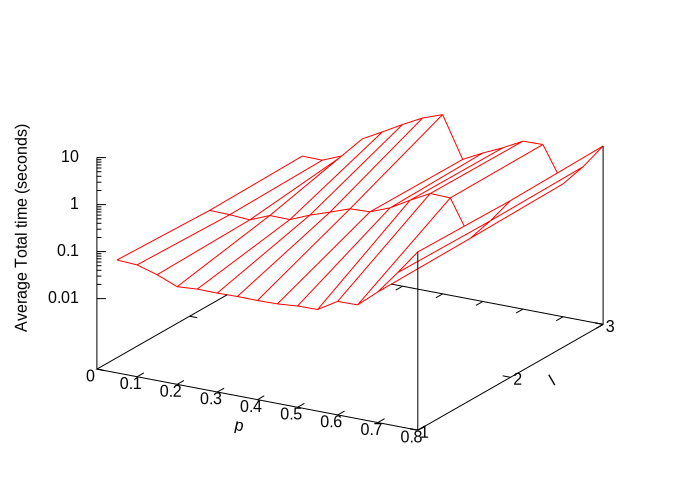
\includegraphics[clip=true, width=0.48\textwidth]{pucs/parameters/k20_n15_l3_time.png}
    }
    &
        \subfigure[] {
        \label{fig:pucs:parameters:small:B}
        \includegraphics[clip=true, width=0.48\textwidth]{pucs/parameters/k20_n20_l3_time.png}
    }
    \end{tabular}   
    \end{center}
    \caption{Gráficos com o tempo de execução médio de acordo com os
    parâmetros $p$ e $l$. A figura~\ref{fig:pucs:parameters:small:A} 
    mostra este valor para uma instância artificial com 15 
    características enquanto a figura~\ref{fig:pucs:parameters:small:B}
    mostra este valor para uma instância de 20 características.}
    \label{fig:pucs:parameters:small}
\end{figure}

A figura~\ref{fig:pucs:parameters:small} mostra como o tempo de 
execução evolui quando aumentamos o valor dos parâmetros $p$ e $l$,
usando como base o algoritmo \algname{UBB}. Nesta figura podemos 
perceber que o parâmetro $l = 3$ aumenta consideravelmente o tempo de 
execução do algoritmo (note a escala logarítmica). Desta maneira, 
repetimos o experimento com valores de $l$ sendo apenas 1 ou 2. Os novos 
resultados são mostrados na figura~\ref{fig:pucs:parameters:small2}, 
que novamente indicam que o aumento do parâmetro $l$ implica em um 
tempo de execução maior. Desta maneira, decidimos que o uso do parâmetro 
$l = 1$ é o mais adequado para o computador que utilizamos. Para o 
parâmetro $p$, basta evitar valores muito pequenos e também muito altos.

\begin{figure}[!ht]
    \begin{center}
    \begin{tabular}{l r}
    \centering
        \subfigure[] {
        \label{fig:pucs:parameters:small2:A}
        \includegraphics[clip=true, width=0.48\textwidth]{pucs/parameters/k20_n12_time.png}
    }
    &
        \subfigure[] {
        \label{fig:pucs:parameters:small2:B}
        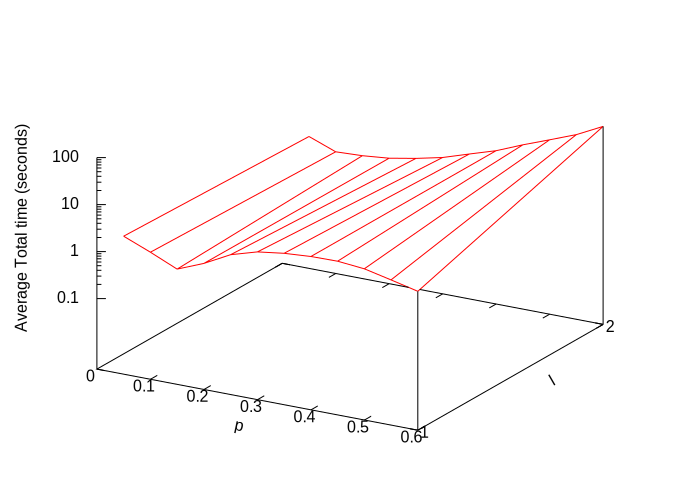
\includegraphics[clip=true, width=0.48\textwidth]{pucs/parameters/k20_n20_time.png}
    }
    \end{tabular}   
    \end{center}
    \caption{Gráficos com o tempo de execução médio de acordo com os
    parâmetros $p$ e $l$. A figura~\ref{fig:pucs:parameters:small2:A} 
    mostra este valor para uma instância artificial com 12 
    características enquanto a figura~\ref{fig:pucs:parameters:small2:B}
    mostra este valor para uma instância de 20 características. O
    algoritmo base utilizado é o \algname{UBB}.}
    \label{fig:pucs:parameters:small2}
\end{figure}


\subsubsection{Instâncias grandes}
Instâncias grandes costumam não ser resolvidas por algoritmos ótimos, 
pois estes demandam recursos computacionais as vezes não disponíveis. 
Desta forma, resolve-se o problema U-Curve com heurísticas, como o 
\algname{Sequential Forward Floating Selection} 
(\algname{SFFS})~\cite{PNK94} ou \algname{Best-First Search} 
(\algname{BFS})~\cite{KJ97}. Para o \algname{PUCS} se tornar uma 
heurística, basta utilizar um algoritmo sub-ótimo como base.

Quando o \algname{PUCS} é ótimo, os parâmetros $p$ e $l$ interferem 
apenas no tempo de execução do algoritmo, mas quando tornamos este 
algoritmo uma heurística, estes parâmetros passam a interferir também
na qualidade das soluções obtidas. Quanto mais fino é o particionamento
feito, mais partes são geradas e resolvidas pelo \algname{PUCS}, e como
cada parte é resolvida com uma chamada do algoritmo base, temos que 
quanto mais granular é o particionamento, mais percorrimentos 
disjuntos acontecerão no reticulado. Desta maneira, quando 
aumentamos o $p$ e $l$, mais buscas são feitas e portanto é 
provável que a solução encontrada seja melhor.

Entretanto, não podemos nos esquecer que estes parâmetros ainda 
influenciam o tempo de execução do algoritmo. Desta maneira não é 
possível aumentar os valores destes parâmetros arbitrariamente até 
atingir a solução com qualidade necessária, e sim aumentar estes 
parâmetros enquanto houverem recursos computacionais compatíveis.

\begin{figure}[!ht]
    \begin{center}
    \begin{tabular}{l r}
    \centering
        \subfigure[] {
        \label{fig:pucs:parameters:big:A}
        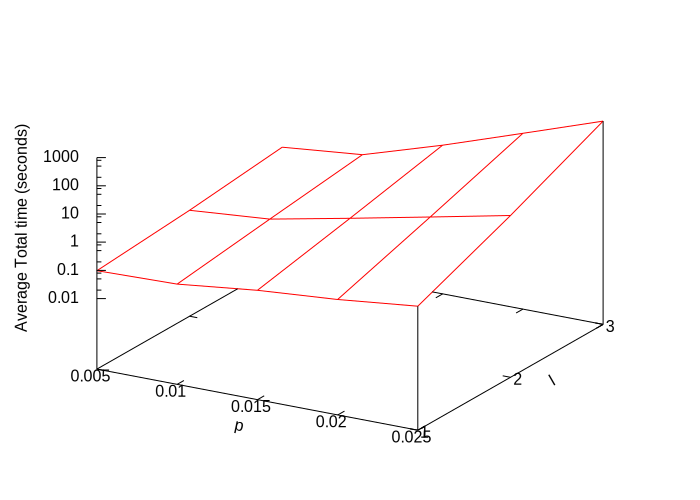
\includegraphics[clip=true, width=0.48\textwidth]{pucs/parameters/n200-20-3_time.png}
    }
    &
        \subfigure[] {
        \label{fig:pucs:parameters:big:B}
        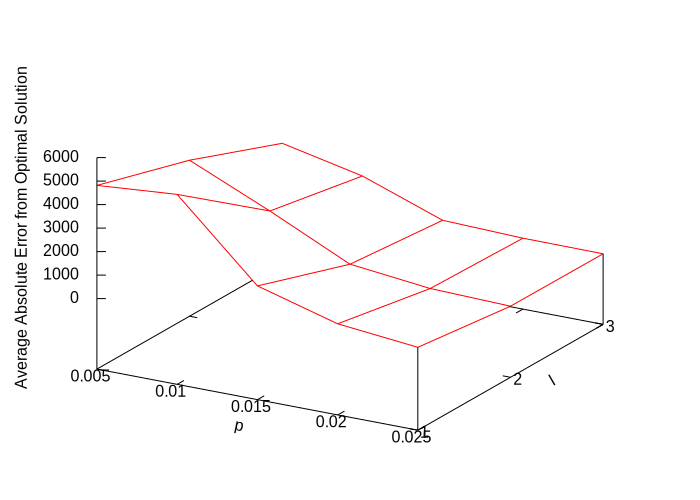
\includegraphics[clip=true, width=0.48\textwidth]{pucs/parameters/n200-20-3_error.png}
    }
    \end{tabular}   
    \end{center}
    \caption{Desempenho do algoritmo \algname{PUCS} para uma 
    instância artificial de 200 características utilizando o 
    \algname{SFFS} como algoritmo base e variando os parâmetros
    $p$ e $l$. A figura~\ref{fig:pucs:parameters:big:A} mostra o tempo
    médio de execução, note que este aumenta quando aumentamos os 
    parâmetros. A figura~\ref{fig:pucs:parameters:big:B} mostra a 
    diferença absoluta média entre o custo do conjunto obtido e do 
    conjunto ótimo.}
    \label{fig:pucs:parameters:big}
\end{figure}

A figura~\ref{fig:pucs:parameters:big} mostra como o tempo de execução
e qualidade da solução se comportam quando aumentamos os valores de 
$p$ e $l$. Confirmando as nossas expectativas, quando amentamos $p$ e
$l$ a qualidade da solução encontrada é mais perto da ótima (o erro 
diminui, no gráfico da figura ~\ref{fig:pucs:parameters:big:B}), e o 
tempo de execução aumenta.

\section{Experimentos com instâncias artificiais}
Nesta seção apresentamos testes feitos com o \algname{PUCS} ao  
solucionar instâncias artificiais do problema U-Curve onde função de 
custo utilizada é a de soma de subconjuntos. Estes testes foram feitos
no arcabouço \toolname{featsel} e foram rodados em uma servidora 
Dell PowerEdge 850, com 64 núcleos e 256 GB de memória RAM.

Como parâmetro $p$ utilizamos um valor tal que o número de variáveis
fixas é sempre 10, o que não compromete a escalabilidade e deve ser 
o suficiente para gerar um número de partes que façam todos os cores
da servidora trabalharem.

\subsection{Experimentos ótimos}
Estes experimentos são feitos em instâncias do problema U-Curve de 
tamanho pequeno, que podem ser resolvidos por algoritmos ótimos. 
Comparamos o \algname{PUCS} com o \algname{UBB}, \algname{PFS} e
também com o algoritmo criado na seção ~\ref{sec:ubbpfs}, o 
\algname{UBB-PFS}. Como parâmetros para estas instâncias utiilizamos 
$p$ tal que número de variáveis fixas é 10, $l = 1$, e o \algname{UBB} 
como algoritmo base.

\begin{table}
\centering
\footnotesize
% \resizebox{\columnwidth}{!}{%

\begin{tabular}{cc c cccc}
\toprule
\multicolumn{2}{c}{Instance} & \phantom{} & \multicolumn{4}{c}{Total time (sec)} \\
\cline{1-2}\cline{4-7}\\
$|S|$ & $2^{|S|}$ && \algname{UBB} & \algname{PFS} & \algname{UBB-PFS} & \algname{PUCS} \\
10 &    1024 &&  0.006 $\pm$ 0.001 & 0.011 $\pm$ 0.002 & 0.022 $\pm$ 0.004 & 0.039 $\pm$ 0.019 \\
11 &    2048 &&  0.007 $\pm$ 0.002 & 0.017 $\pm$ 0.004 & 0.026 $\pm$ 0.005 & 0.045 $\pm$ 0.022 \\
12 &    4096 &&  0.009 $\pm$ 0.003 & 0.029 $\pm$ 0.009 & 0.033 $\pm$ 0.008 & 0.048 $\pm$ 0.024 \\
13 &    8192 &&  0.013 $\pm$ 0.006 & 0.054 $\pm$ 0.016 & 0.047 $\pm$ 0.014 & 0.053 $\pm$ 0.021 \\
14 &   16384 &&  0.026 $\pm$ 0.012 & 0.103 $\pm$ 0.035 & 0.074 $\pm$ 0.017 & 0.057 $\pm$ 0.024 \\
15 &   32768 &&  0.048 $\pm$ 0.027 & 0.195 $\pm$ 0.080 & 0.116 $\pm$ 0.044 & 0.056 $\pm$ 0.025 \\
16 &   65536 &&  0.097 $\pm$ 0.055 & 0.354 $\pm$ 0.176 & 0.198 $\pm$ 0.089 & 0.090 $\pm$ 0.080 \\
17 &  131072 &&  0.142 $\pm$ 0.120 & 0.676 $\pm$ 0.375 & 0.350 $\pm$ 0.200 & 0.255 $\pm$ 0.276 \\
18 &  262144 &&  0.319 $\pm$ 0.228 & 1.512 $\pm$ 0.764 & 0.751 $\pm$ 0.338 & 0.680 $\pm$ 0.592 \\
19 &  524288 &&  0.684 $\pm$ 0.464 & 2.875 $\pm$ 1.554 & 1.387 $\pm$ 0.707 & 1.492 $\pm$ 1.323 \\
20 & 1048576 &&  1.249 $\pm$ 0.975 & 5.295 $\pm$ 3.509 & 2.594 $\pm$ 1.569 & 2.701 $\pm$ 2.908 \\
21 & 2097152 &&  2.671 $\pm$ 1.948 & 11.136 $\pm$ 6.947 & 5.460 $\pm$ 3.392 & 6.118 $\pm$ 5.961 \\
22 & 4194304 &&  5.420 $\pm$ 4.202 & 19.825 $\pm$ 14.519 & 9.709 $\pm$ 7.319 & 11.729 $\pm$ 11.613 \\
\bottomrule
\end{tabular}
\caption{Comparação de tempo de execução de algoritmos ótimos para o
problema U-Curve. O \algname{PUCS} foi o segundo algoritmo mais lento,
sendo mais rápido do que o \algname{PFS} apenas.}
\label{tab:pucs:small:time}
% }
\end{table}


A tabela ~\ref{tab:pucs:small:time} mostra o tempo de execução médio
dos algoritmos \algname{UBB}, \algname{PFS}, \algname{UBB-PFS} e
\algname{PUCS}. O desempenho em tempo do \algname{PUCS} foi similar
ao \algname{UBB-PFS}, porém só foi melhor que o \algname{PFS}. A tabela 
~\ref{tab:pucs:small:cost} mostra, para os mesmos algoritmos, o número 
médio de chamadas da função custo. O \algname{PUCS} computou menos nós 
do que o \algname{UBB}, e computou pouco mais nós do que o \algname{PFS} 
e \algname{UBB-PFS}.


\begin{table}
\centering
\footnotesize
\resizebox{\columnwidth}{!}{%
\begin{tabular}{cc c cccc}
\toprule
\multicolumn{2}{c}{Instance} & \phantom{} & \multicolumn{4}{c}{\# Calls of cost function} \\
\cline{1-2}\cline{4-7}\\
$|S|$ & $2^{|S|}$ && UBB & PFS & UBB-PFS & PUCS \\
 % 1 &       2 && 2.0 $\pm$  0.0 &  2.0 $\pm$  0.0 &  2.0 $\pm$  0.0 &  5.0 $\pm$  0.0 \\
 % 2 &       4 && 3.8 $\pm$  0.4 &  3.9 $\pm$  0.2 &  3.8 $\pm$  0.4 &  7.4 $\pm$  0.9 \\
 % 3 &       8 && 6.9 $\pm$  1.3 &  7.7 $\pm$  0.5 &  6.9 $\pm$  1.3 & 15.0 $\pm$  3.2 \\
 % 4 &      16 && 13.1 $\pm$  3.5 & 13.1 $\pm$  2.9 & 13.1 $\pm$  3.5 & 28.6 $\pm$  8.1 \\
 % 5 &      32 && 25.0 $\pm$  8.2 & 25.4 $\pm$  5.1 & 24.4 $\pm$  7.5 & 50.3 $\pm$ 14.4 \\
 % 6 &      64 && 50.7 $\pm$ 16.7 & 49.6 $\pm$ 13.9 & 49.3 $\pm$ 14.4 & 97.8 $\pm$ 32.9 \\
 % 7 &     128 && 101.6 $\pm$ 34.2 & 80.2 $\pm$ 29.3 & 95.1 $\pm$ 24.9 & 167.4 $\pm$ 57.6 \\
 % 8 &     256 && 166.2 $\pm$ 89.6 & 173.0 $\pm$ 33.9 & 162.7 $\pm$ 69.7 & 274.1 $\pm$ 136.8 \\
 % 9 &     512 && 356.2 $\pm$ 193.1 & 313.0 $\pm$ 91.9 & 323.1 $\pm$ 126.6 & 472.8 $\pm$ 285.4 \\
10 &    1024 && 668.2 $\pm$ 359.2 & 614.2 $\pm$ 162.7 & 630.3 $\pm$ 235.9 & 753.6 $\pm$ 493.6 \\
11 &    2048 && 1171.5 $\pm$ 742.5 & 1139.2 $\pm$ 354.0 & 1174.8 $\pm$ 499.3 & 1305.0 $\pm$ 881.8 \\
12 &    4096 && 2611.6 $\pm$ 1528.5 & 2137.1 $\pm$ 793.3 & 2271.2 $\pm$ 894.1 & 2370.5 $\pm$ 1615.7 \\
13 &    8192 && 4583.2 $\pm$ 2910.2 & 4218.9 $\pm$ 1306.7 & 4308.7 $\pm$ 1732.2 & 4780.0 $\pm$ 2797.7 \\
14 &   16384 && 10781.4 $\pm$ 5565.5 & 8211.1 $\pm$ 3054.5 & 9050.4 $\pm$ 2638.1 & 7050.8 $\pm$ 4755.7 \\
15 &   32768 && 20891.9 $\pm$ 12757.0 & 15134.0 $\pm$ 6528.5 & 15900.7 $\pm$ 6927.4 & 14080.1 $\pm$ 11373.1 \\
16 &   65536 && 43529.6 $\pm$ 25318.9 & 26447.0 $\pm$ 13446.1 & 28783.6 $\pm$ 12934.2 & 26001.3 $\pm$ 21699.6 \\
17 &  131072 && 65301.0 $\pm$ 56215.8 & 49694.5 $\pm$ 27621.8 & 51032.5 $\pm$ 29984.3 & 50145.2 $\pm$ 46799.0 \\
18 &  262144 && 145594.5 $\pm$ 103597.8 & 105603.1 $\pm$ 52652.2 & 110538.0 $\pm$ 51589.7 & 111296.6 $\pm$ 84922.4 \\
19 &  524288 && 313096.0 $\pm$ 209913.1 & 194572.5 $\pm$ 104802.3 & 204604.5 $\pm$ 100305.4 & 233717.7 $\pm$ 186182.0 \\
20 & 1048576 && 578319.0 $\pm$ 445912.2 & 340052.5 $\pm$ 221271.6 & 362007.0 $\pm$ 207411.2 & 387082.0 $\pm$ 389417.4 \\
% 21 & 2097152 && 1208939.1 $\pm$ 867260.3 & 699906.1 $\pm$ 437209.1 & 726193.9 $\pm$ 420497.8 & 854293.9 $\pm$ 779635.6 \\
% 22 & 4194304 && 2375634.9 $\pm$ 1826536.5 & 1195439.1 $\pm$ 881956.5 & 1253704.3 $\pm$ 847533.7 & 1640138.3 $\pm$ 1547703.6 \\
\bottomrule
\end{tabular}
}
\caption{Comparação de número de chamadas da função custo em algoritmos
ótimos do problema U-Curve. O \algname{PUCS} faz menos chamadas da
função custo que o \algname{UBB}, porém faz mais chamadas do que o 
\algname{PFS} e \algname{PFS-UBB}.}
\label{tab:pucs:small:cost}
\end{table}

\subsection{Experimentos sub-ótimos}
Estes experimentos foram feitas em instâncias do problema U-Curve que
são grandes e geralmente não podem ser resolvidas por algoritmos ótimos.
Comparamos o desempenho do \algname{PUCS} contra as heurísticas 
\algname{SFFS}~\cite{PNK94} e \algname{BFS}~\cite{KJ97}. Utilizamos
como parâmetros $p$ tal que o número de variáveis fixas é 10, $l = 1$,
e, como algoritmo base, utilizamos a heurística 
\algname{Sequential Forward Selection} \algname{SFS}~\cite{Whi71}.

A figura~\ref{fig:pucs:big:time} compara o tempo de execução do 
\algname{PUCS} com heurísticas. Apesar do desvio padrão grande, podemos
observar que, com os parâmetros citados, o \algname{PUCS} foi o 
algoritmo mais lento entre os testados. A 
figura~\ref{fig:pucs:big:correctness} mostra para cada uma das três
heurísticas testadas a proporção de vezes em que o algoritmo achou a
solução de menor custo entre os três. Neste teste, o \algname{PUCS}
teve proporção de melhor solução de 100\% para todos os tamanhos
de instâncias testadas, isto é, a solução encontrada por este algoritmo
teve custo sempre menor ou igual do que as soluções encontradas
pelo \algname{SFFS} e \algname{BFS}.


\begin{figure}[!ht]
    \begin{center}
    \begin{tabular}{l r}
    \centering
        \subfigure[] {
        \label{fig:pucs:big:time}
        \includegraphics[clip=true, width=0.5\textwidth]{pucs/experiments/time_sffs_bfs_pucs.png}
    }
    &
        \subfigure[] {
        \label{fig:pucs:big:correctness}
        \includegraphics[clip=true, width=0.5\textwidth]{pucs/experiments/correctness_sffs_bfs_pucs.png}
    }
    \end{tabular}   
    \end{center}
    \caption{Comparação entre os algoritmos \algname{SFFS}, 
    \algname{BFS} e \algname{PUCS}. A figura~\ref{fig:pucs:big:time} 
    mostra o tempo médio de execução dos algoritmos. A 
    figura~\ref{fig:pucs:big:correctness} mostra a proporção de vezes
    em que cada algoritmo achou a melhor resposta entre os três.}
    \label{fig:pucs:big}
\end{figure}

\subsection{Comentários sobre os experimentos}
Os experimentos ótimos com o \algname{PUCS} mostraram que este algoritmo
possui tempo de execução menor do que o \algname{PFS} e pouco maior do
que \algname{UBB-PFS}. Quanto ao número de chamadas da função de custo,
o \algname{PUCS} teve desempenho melhor do que o \algname{UBB}, e 
um desempenho similar ao \algname{UBB-PFS}. Em resumo, o \algname{PUCS}
é um algoritmo tão competitivo quanto o \algname{UBB-PFS} para estas
instâncias.

O \algname{PUCS} se mostrou mais interessante quando 
utilizado para resolver instâncias de maneira sub-ótima. Para estes 
experimentos, este algoritmo teve tempo médio de execução pior do que 
as outras heurísticas, porém a qualidade da solução encontrada foi 
sempre melhor ou igual a solução dos outros algoritmos. Logo este 
algoritmo é recomendável para problemas em que o recurso de tempo é
grande o suficiente. Além disso, o pior tempo de execução observado
na figura~\ref{fig:pucs:big:time} foi medido com parâmetros $p$ e $l$
fixos, e como vimos na seção~\ref{sec:pucs:parameters}, podemos diminuir
o tempo de execução ao diminuir o valor destes parâmetros.

Por ser um algoritmo paralelo com pouco compartilhamento de memória, 
esperamos que o desempenho do \algname{PUCS} melhore (até algum ponto
de saturação) quando aumentamos os recursos de processadores da máquina
utilizada. Desta maneira, respeitando os limites da paralelização na 
máquina, com maiores recursos de tempo e processamento é esperado que 
possamos aumentar os parâmetros $p$ e $l$, conseguindo melhores 
soluções. Em uma máquina hipoteticamente tão rápida quanto necessário,
podemos aumentar a qualidade das soluções ao aumentar os valores dos
parâmetros até que, no limite, o \algname{PUCS} se torne ótimo.
